\chapter{Description}

The interpreter pattern consists of different classes. There is one class for each symbol. These symbols can either be \textit{terminal} or \textit{nonterminal}. 


\section{Grammar}

In order to understand the Interpreter Pattern, you also need to understand the basic concepts of grammar. A grammar is basically \textbf{the language of languages}. Every language must have a grammar to determine its structure. There's different notations and symbols used in a grammar. For example, there are multiple symbols in a grammar: \textit{Nonterminal} and \textit{terminal}. There are also different notations like: \textit{Backus-Naur Form (BNF)} or \textit{Extended Backus-Naur Form (EBNF)}.


\subsection{Terminal Symbols}
\label{sec:terminal-symbols}

Terminal symbols cannot be replaced by production rules. All terminal symbols define an alphabet, of which sentences or words consist of.

To phrase it differently: Terminal symbols are basically the leaf nodes of a syntax tree. Here's an example of what this could look like: 

\begin{figure}[H]
    \centering
        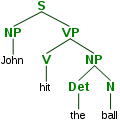
\includegraphics[width=0.4\textwidth]{figures/parse-tree.png}
        \caption{Parse Tree}
\end{figure}

The terminal symbols here are: \textit{John}, \textit{hit}, \textit{the} and \textit{ball}.

Terminal symbols are also often used for punctuation marks or keywords in programming languages. For example in C\#, you could use: \textit{for}, \textit{while}, \textit{var}, \textit{if} and every other keyword.

% https://de.wikipedia.org/wiki/Syntaxbaum
% https://de.wikipedia.org/wiki/Terminalsymbol
% https://en.wikipedia.org/wiki/Terminal_and_nonterminal_symbols


\subsection{Nonterminal Symbols}
\label{sec:nonterminal-symbols}

Nonterminal symbols are the opposite of terminal symbols. These are symbols which can be replaced. A formal grammar includes a \textit{start symbol} (which is also a nonterminal symbol) and a set of nonterminal symbols. Then, with the production rules, every sentence in a language can be derived from them. Usually, terminal symbols will be used to replace the nonterminal ones. 

Let's look at the example again: 

\begin{figure}[H]
    \centering
        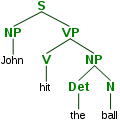
\includegraphics[width=0.4\textwidth]{figures/parse-tree.png}
        \caption{Parse Tree}
\end{figure}

The parse tree is the entire structure, starting from \textit{S} and ending in each of the leaf nodes (John, hit, the, ball). The following abbreviations are used in the tree:

\begin{itemize}
    \item \textit{S} for sentence
    \item \textit{NP} for noun phrase
    \item \textit{VP} for verb phrase
    \item \textit{V} for verb
    \item \textit{D} for determiner
    \item \textit{N} for noun
\end{itemize}

There is also a differentiation between root node, branch node and leaf node. A \textit{root node}, is a node that doesn't any predecessors. In this example \textit{S} is the root node. Within a sentence there can also only ever be one root node. A \textit{branch node} is a parent node, that connects two or more child nodes, which can again be branch or leaf nodes. \textit{VP} and \textit{NP} are the branch nodes in this example. A \textit{leaf node} does not have any other child nodes apart from the terminal symbols. 

There are also multiple ways of visualizing this parse tree. See section \ref{sec:syntax-tree} fore more information.

% https://en.wikipedia.org/wiki/Terminal_and_nonterminal_symbols
% https://de.wikipedia.org/wiki/Nichtterminalsymbol



\subsection{Production Rules}
\label{sec:production-rules}

A grammar is defined by production rules, which specify, which symbols can be replaced with which symbols. Each rule has a \textit{head}, or \textit{left-hand-side}, and \textit{body}, or \textit{right-hand-side}. 

Rules are often written in the \textit{head → body} format. For example the rule \textit{a → b} specifies that \textit{a} can be replaced by \textit{b}. 

\subsubsection{Example}

Let's say you have your custom alphabet. You alphabet consists of the following: 

\begin{itemize}
    \item Nonterminal Symbols: A, B, C
    \item Terminal Symbols: D, E, F
\end{itemize}

So we defined the symbols, but we are missing something. We cannot define any sentences or words with this. This is were the production rules can be used. So we can for example define that the nonterminal symbol \textit{A} can be replaced with the terminal symbols \textit{E} and \textit{F}. This can then also be done for every other nonterminal symbol and then you have your basic grammar. 

\begin{verbatim}
    A → E, F
    B → D, E, F
    C → F
\end{verbatim}

% https://en.wikipedia.org/wiki/Terminal_and_nonterminal_symbols
% https://www.youtube.com/watch?v=Rhqk9HYiB7Q



\section{Syntax Tree}
\label{sec:syntax-tree}

Parse trees are also often known as \textit{derivation trees} or \textit{(concrete) syntax tree}. Parse trees is a tree-like data structure that represents a concrete representation of the input. Parse trees retain all of the information of the input. Here we again have a start symbol \textit{S}, nonterminal and terminal symbols as mentioned in section \ref{sec:production-rules}. 

\begin{figure}[H]
    \centering
        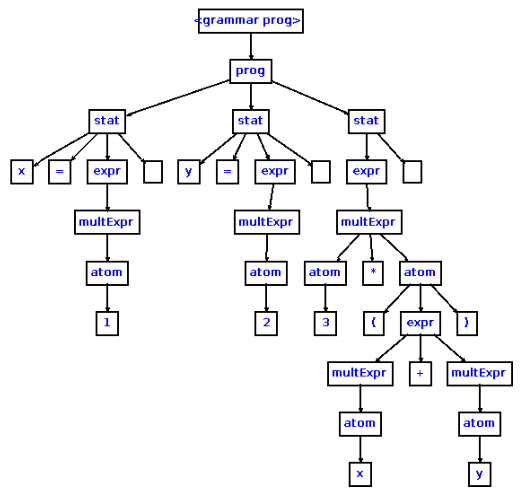
\includegraphics[width=0.6\textwidth]{figures/parse_tree.png}
        \caption{Parse Tree}
\end{figure}

As you can see, this parse tree contains all the meta data, which might not be needed. For example you could simply remove nonterminal symbols like \textit{atom}, because they only have one terminal expression as child. This is where the \nameref{sec:abstract-syntax-tree} can be used.

% https://de.wikipedia.org/wiki/Syntaxbaum
% https://en.wikipedia.org/wiki/Parse_tree
% https://stackoverflow.com/a/10177369




\section{Abstract Syntax Tree}
\label{sec:abstract-syntax-tree}

The \textit{Abstract Syntax Tree} (AST) is an abstract representation of the input. You'll notice that most of the nonterminal expressions are not present anymore, because unimportant translations have been removed.\textbf{ In other words, an \textit{Abstract Syntax Tree} highlights the structure of a language and not the grammar (like the syntax tree)}. 

\begin{figure}[H]
    \centering
        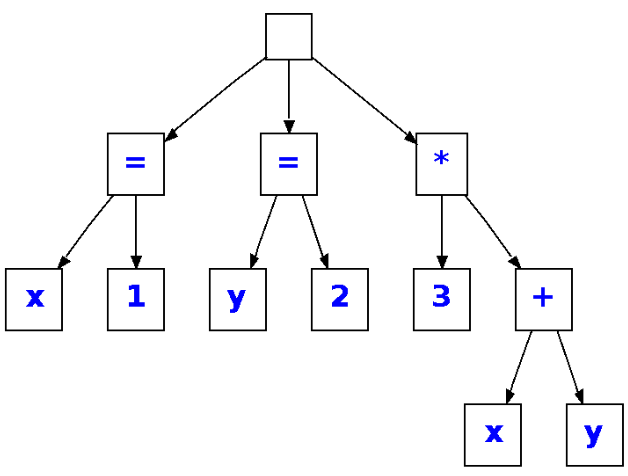
\includegraphics[width=0.6\textwidth]{figures/ast.png}
        \caption{AST}
\end{figure}

When you compare it to the parse tree, you can already see, that it's much easier to understand. Let's look at another example. You can also parse source code, like this simple JavaScript function, which just does a mathematical calculation based on the input. 

\begin{verbatim}
function foo(x) {
    if (x > 10) {
        var a = 2;
        return a * x;
    }

    return x + 10;
}
\end{verbatim}

The resulting \textit{Abstract Syntax Tree} could look like this. 

\begin{figure}[H]
    \centering
        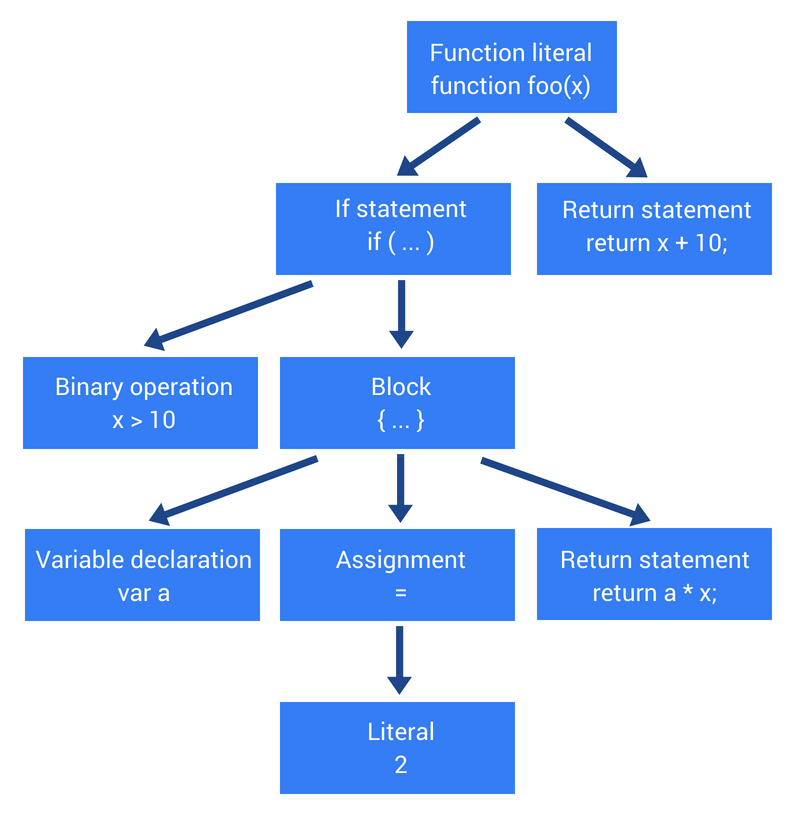
\includegraphics[width=0.5\textwidth]{figures/javascript_ast.png}
\end{figure}

This AST has been simplified for visualization purposes. The actual AST would be much more complex and contain more data. There's a cool project, where you can show the actual AST of a JavaScript program: https://astexplorer.net/

\subsection{Usage in Compilers}

\textit{Abstract Syntax Trees} are also often used, to represent the structure of the program code in various computer languages. An AST is usually the result of the analysis of the source code by the compiler. It does also often serve as an intermediate representation of the program, which is needed for the compiler. 

For example the compiler \href{https://llvm.org/}{LLVM} uses their own intermediate language (or AST), which can then be used by other programs. This brings the big advantage, that other programs can convert their AST, to be able to compile their code. Renowned programming languages that use LLVM as their backend are RustLang, C++, C and even Java. 

\subsubsection{Motivation}

An AST has several properties that aid the further steps of the compilation process:

\begin{itemize}
    \item An AST can be edited and enhanced with information such as properties or annotations.
    
    \begin{itemize}
        \item This cannot be done with source code, because then it would need to be changed. 
    \end{itemize}

    \item An AST doesn't include punctuation and delimiters (braces, semicolons, parentheses, ...), because they are not needed.
\end{itemize}

During the first stage, the syntax analysis, the compiler produces a parse tree. This parse tree will then be converted to an AST. This will almost always lead to a more efficient compiler. An AST has also the advantage that it has a smaller height and smaller number of elements. 

\subsubsection{Design}

The design of the \textit{Abstract Syntax Tree} is also a crucial part of the compiler design. This design is often closely linked with the design of a compiler and its expected features. 

Core requirements must include the following: 

\begin{itemize}
    \item Variable types must be preserved, as well as the location of each declaration in source code. 
    \item The order of executable statements must be explicitly represented and well defined.
    \item Left and right components of binary operations must be stored and correctly identified.
    \item Identifiers and their assigned values must be stored for assignment statements.
\end{itemize}

These items can help designing the data structure of the AST. You also want to support the verification of the source code via the compiler. This can be done by unparsing the AST into source code form. The resulting source code should be similar to the original. 

% https://stackoverflow.com/a/10177369
% https://en.wikipedia.org/wiki/Abstract_syntax_tree
% https://blog.sessionstack.com/how-javascript-works-parsing-abstract-syntax-trees-asts-5-tips-on-how-to-minimize-parse-time-abfcf7e8a0c8




\section{Backus–Naur form}
\label{sec:backus-naur-form}

This is a notation technique, that is often used to describe the syntax of languages. 

A BNF specification is a set of derivation rules, which can be written like this: 

\begin{verbatim}
<symbol> ::= __expression__
\end{verbatim}

Here the \textit{symbol} is \textit{nonterminal} and the \textit{expression} consists of one or more \textit{terminal symbols}. The \textit{::=} means that the symbol on the left must be replaced with one of the symbols on the right. The BNF also uses different production rules to map the nonterminal to the terminal symbols. This has already been discussed in section \ref{sec:terminal-symbols} and \ref{sec:nonterminal-symbols}.

\subsection{Example}

For example, this is how a simple terminal symbol could look like. A digit without zero, can either be 1, 2, 3 and so on. 

\begin{verbatim}
<Digit without Zero> ::= 1 | 2 | 3 | 4 | 5 | 6 | 7 | 8 | 9
\end{verbatim}

You can also use a sequence, with multiple terminal and nonterminal symbols: 

\begin{verbatim}
<Digit>             ::= 0 | <Digit without Zero>
<Twodigit Number>   ::= <Digit without Zero> <Digit>
<Ten to Nineteen>   ::= 1 <Digit>
<Fourtytwo>         ::= 42
\end{verbatim}
    
Here \textit{Digit} can either be 0 or a digit without zero. If you don't specify a separator, it'll be concatenated. 

% https://de.wikipedia.org/wiki/Backus-Naur-Form


\section{Reverse Polish Notation}
\label{sec:reverse-polish-notation}

This is another notation, which is also known as \textit{polish postfix notation}. It's a mathematical notation where the operators follow their operands. 

For example, a normal addition looks like this: \textbf{3 + 4}. In the polish postfix notation, you move the operator to the end. This will look like this: \textbf{3 4 +}. If you take a more advanced example like \textbf{3 - 4 + 5}, this can be written as \textbf{3 4 - 5 +}. 4 is first subtracted from 3, then 5 is added to it. 

However, there is one big advantage: the \textit{Reverse Polish Notation} removes the need for parentheses. While \textbf{3 - 4 × 5} can also be written as \textbf{3 - (4 × 5)}, that means something quite different than \textbf{(3 - 4) × 5}. In \textit{Reverse Polish Notation}, the former could be written \textbf{3 4 5 - ×} and the latter \textbf{3 4 - 5 ×}. 

% https://en.wikipedia.org/wiki/Reverse_Polish_notation